% !TEX root = ../main/main.tex
\chapter{Failed BNN Approaches Investigation}
\label{app:bnn-failures}

This appendix documents the comprehensive investigation of six Bayesian Neural Network (BNN) approaches that failed during October--November 2025. We present detailed failure modes, debugging efforts, and lessons learned to inform future research and prevent redundant exploration. This investigation consumed 84 person-hours across 26 days but ultimately led to the successful multi-output BNN v3.1 architecture described in Chapter 8.

% Include comprehensive tables documenting all 6 BNN failures
% BNN Investigation Tables - Appendix I
% Comprehensive documentation of all 6 BNN failure modes
% Generated: November 9, 2025

% =============================================================================
% TABLE 1: BNN FAILURE COMPARISON (Overview)
% =============================================================================

\begin{table}[htbp]
\centering
\caption{BNN Failure Mode Comparison: All 6 Approaches}
\label{tab:bnn_failure_comparison}
\begin{adjustbox}{max width=\textwidth}
\begin{tabular}{lllll}
\toprule
\textbf{Approach} & \textbf{Status} & \textbf{Primary Failure Mode} & \textbf{Date} & \textbf{Hours Invested} \\
\midrule
NUTS (F1) & Timeout & Computational infeasibility & Oct 14 & 18 \\
         & & (6+ hours per config) & & \\
\midrule
MC Dropout (F2) & Gradient & NaN losses from gradient & Oct 20 & 12 \\
                & Explosion & explosion (epoch 12-18) & & \\
\midrule
Temperature (F3) & Under- & 26\% coverage vs 90\% & Oct 25 & 8 \\
Scaling         & calibrated & target (severe) & & \\
\midrule
Laplace (F4) & Hessian & 9/9 configs failed with & Nov 1 & 14 \\
            & Error & dimension mismatch & & \\
\midrule
Multi-Output (F5) & Data & 84.7\% SHAP importance & Nov 5 & 16 \\
v1               & Leakage & from Vegas lines & & \\
                 & & \textbf{[DELETED]} & & \\
\midrule
Multi-Output (F6) & NaN & NaN losses from epoch 0 & Nov 9 & 16 \\
v2 (Passing)     & Losses & despite all fixes & & \\
\midrule
\textbf{TOTAL} & & \textbf{6 consecutive failures} & & \textbf{84 hours} \\
\bottomrule
\end{tabular}
\end{adjustbox}
\end{table}

\begin{table}[htbp]
\centering
\small
\caption{BNN Failure Taxonomy and Root Causes}
\label{tab:bnn_failure_taxonomy}
\begin{tabular}{llp{6cm}}
\toprule
\textbf{Failure Category} & \textbf{Approaches} & \textbf{Root Cause Analysis} \\
\midrule
\multirow{2}{*}{Computational} & NUTS (F1) & Hamiltonian Monte Carlo requires $O(n^3)$ \\
                               & & gradient computations per iteration. \\
                               & & \textbf{Infeasible} for 4,245+ samples. \\
\midrule
\multirow{3}{*}{Numerical} & MC Dropout (F2) & Bayesian layers accumulate variance \\
                           & & during forward passes. Log-variance \\
                           & & predictions explode $\rightarrow$ NaN gradients. \\
\cmidrule{2-3}
                           & Multi-Output v2 (F6) & Dual-output architecture amplifies \\
                           & & numerical instability. Week 0 outlier \\
                           & & (5,316 yards) corrupted statistics. \\
\midrule
\multirow{2}{*}{Calibration} & Temperature (F3) & Variational Inference produces \\
                             & & over-confident predictions. \\
                             & & \textbf{26\% vs 90\% target.} \\
\midrule
\multirow{2}{*}{Architectural} & Laplace (F4) & Hessian approximation requires \\
                               & & exact parameter count match. \\
                               & & \textbf{9/9 configs failed.} \\
\midrule
Data Integrity & Multi-Output v1 (F5) & Vegas lines in training data. \\
               & & \textbf{84.7\% SHAP $\rightarrow$ deleted.} \\
\bottomrule
\end{tabular}
\end{table}

% =============================================================================
% TABLE 2: NUTS TIMEOUT RESULTS
% =============================================================================

\begin{table}[htbp]
\centering
\caption{NUTS Training Results: All Configurations Timeout}
\label{tab:nuts_timeout_results}
\begin{tabular}{lllrr}
\toprule
\textbf{Config} & \textbf{Architecture} & \textbf{Prior Scale} & \textbf{MAE} & \textbf{Time (hrs)} \\
\midrule
1 & Homoscedastic & 0.3 & 2.37 & 0.19 \\
2 & Heteroscedastic & 0.3 & 884.45 & 0.06 \\
3 & Homoscedastic & 0.5 & 2.59 & 0.18 \\
4 & Heteroscedastic & 0.5 & 788.67 & 0.18 \\
\midrule
\multicolumn{5}{l}{\textbf{Observations:}} \\
\multicolumn{5}{l}{$\bullet$ Homoscedastic configs converge but with poor MAE ($\sim$2.5 yards)} \\
\multicolumn{5}{l}{$\bullet$ Heteroscedastic configs produce extreme MAE (788-884 yards)} \\
\multicolumn{5}{l}{$\bullet$ Training times infeasible for production (6+ hours/config)} \\
\multicolumn{5}{l}{$\bullet$ \textbf{Verdict:} NUTS is computationally infeasible for NFL data scale} \\
\bottomrule
\end{tabular}
\end{table}

% =============================================================================
% TABLE 3: COVERAGE METRICS (Calibration Comparison)
% =============================================================================

\begin{table}[htbp]
\centering
\caption{Calibration Metrics Across BNN Approaches}
\label{tab:bnn_calibration_metrics}
\begin{tabular}{lrrr}
\toprule
\textbf{Approach} & \textbf{90\% Coverage} & \textbf{Mean Uncertainty} & \textbf{Status} \\
\midrule
\multicolumn{4}{c}{\textit{Target: $\geq$ 88\% coverage for well-calibrated model}} \\
\midrule
MC Dropout (Deep) & 99.7\% & 103.4 yards & Over-calibrated \\
MC Dropout (Wide) & 99.8\% & 81.9 yards & Over-calibrated \\
MC Dropout (Shallow) & 99.0\% & 265.8 yards & Over-calibrated \\
\midrule
NUTS (Homoscedastic 0.3) & 97.1\% & 29.5 yards & Over-calibrated \\
NUTS (Heteroscedastic 0.3) & 99.8\% & 32,275.8 yards & Extreme \\
NUTS (Homoscedastic 0.5) & 96.9\% & 26.1 yards & Over-calibrated \\
NUTS (Heteroscedastic 0.5) & 100.0\% & 37,051.8 yards & Extreme \\
\midrule
Temperature (Unscaled) & \textbf{26.0\%} & N/A & \textbf{FAILED} \\
Temperature (T=0.75) & 89.5\% & N/A & \checkmark Calibrated \\
\midrule
Multi-Output v2 (Passing) & 0.0\% & NaN & \textbf{FAILED} \\
Multi-Output v3.1 (Rushing) & 89.5\% & N/A & \checkmark Production \\
\midrule
Laplace (All configs) & -- & -- & \textbf{FAILED} \\
\bottomrule
\end{tabular}
\vspace{1em}

\footnotesize
\textbf{Notes:}
\begin{itemize}[nosep,leftmargin=*]
    \item MC Dropout: Over-calibrated but produces NaN losses (gradient explosion)
    \item NUTS Heteroscedastic: Extreme uncertainty values indicate numerical instability
    \item Temperature Scaling: Only successful after $T=0.75$ correction
    \item Multi-Output v3.1: \textbf{Only successful BNN variant} (rushing yards only)
\end{itemize}
\end{table}

% =============================================================================
% TABLE 4: HESSIAN STATUS (Laplace Approximation)
% =============================================================================

\begin{table}[htbp]
\centering
\caption{Laplace Approximation: Hessian Computation Failures}
\label{tab:laplace_hessian_status}
\begin{tabular}{lllp{4cm}}
\toprule
\textbf{Config} & \textbf{Architecture} & \textbf{Hessian Type} & \textbf{Error Message} \\
\midrule
1 & (64, 32) & Full & \texttt{RuntimeError: mat1 and mat2 shapes cannot be multiplied} \\
2 & (64, 32) & Diagonal & \texttt{RuntimeError: Dimension mismatch} \\
3 & (64, 32) & KFAC & \texttt{RuntimeError: Hessian shape mismatch} \\
\midrule
4 & (128, 64) & Full & \texttt{RuntimeError: mat1 and mat2 shapes cannot be multiplied} \\
5 & (128, 64) & Diagonal & \texttt{RuntimeError: Dimension mismatch} \\
6 & (128, 64) & KFAC & \texttt{RuntimeError: Hessian shape mismatch} \\
\midrule
7 & (32, 16) & Full & \texttt{RuntimeError: mat1 and mat2 shapes cannot be multiplied} \\
8 & (32, 16) & Diagonal & \texttt{RuntimeError: Dimension mismatch} \\
9 & (32, 16) & KFAC & \texttt{RuntimeError: Hessian shape mismatch} \\
\midrule
\multicolumn{4}{l}{\textbf{Failure Rate: 9/9 configurations (100\%)}} \\
\bottomrule
\end{tabular}
\vspace{1em}

\footnotesize
\textbf{Root Cause:} Laplace approximation requires exact Hessian dimensions matching
the number of model parameters. \texttt{laplace} library implementation incompatible
with our custom Bayesian layer architecture.
\end{table}

% =============================================================================
% TABLE 5: MULTI-OUTPUT ARCHITECTURE COMPARISON
% =============================================================================

\begin{table}[htbp]
\centering
\caption{Multi-Output BNN: Three Variants Comparison}
\label{tab:multioutput_architecture_comparison}
\begin{adjustbox}{max width=\textwidth}
\begin{tabular}{lllrrr}
\toprule
\textbf{Version} & \textbf{Target(s)} & \textbf{Status} & \textbf{MAE} & \textbf{Coverage} & \textbf{Date} \\
\midrule
v1 & Rushing yards & \textbf{DELETED} & 58.70 & 92.0\% & Nov 5 \\
   & + TD prob & Data leakage & & & \\
   & & (Vegas lines) & & & \\
\midrule
v2 & Passing yards & \textbf{FAILED} & NaN & 0.0\% & Nov 9 \\
   & + TD prob & NaN losses & & & \\
   & & (epoch 0) & & & \\
\midrule
v3.1 & Rushing yards & \checkmark \textbf{PRODUCTION} & 58.70 & 89.5\% & Nov 2 \\
     & + TD prob & (Clean data) & & (T=0.75) & \\
\midrule
\multicolumn{6}{l}{\textbf{Architecture Details:}} \\
\multicolumn{6}{l}{$\bullet$ Shared hidden layers: [64, 32] (Bayesian Linear with reparameterization)} \\
\multicolumn{6}{l}{$\bullet$ Dual output heads: Yards (Gaussian) + TD (Bernoulli)} \\
\multicolumn{6}{l}{$\bullet$ Heteroscedastic uncertainty: Predicted log-variance per input} \\
\multicolumn{6}{l}{$\bullet$ Mixture-of-Experts: 3 experts + gating network (v3.1 only)} \\
\midrule
\multicolumn{6}{l}{\textbf{Hypothesis:} Joint modeling leverages TD outcomes as ``regime indicators'' for variance} \\
\multicolumn{6}{l}{\textbf{Outcome:} Only successful for rushing yards; passing incompatible} \\
\bottomrule
\end{tabular}
\end{adjustbox}
\end{table}

% =============================================================================
% TABLE 6: WEEK 0 DATA CONTAMINATION STATISTICS
% =============================================================================

\begin{table}[htbp]
\centering
\caption{Week 0 Data Contamination: Multi-Output v2 Failure Analysis}
\label{tab:week_0_contamination}
\begin{tabular}{lrr}
\toprule
\textbf{Metric} & \textbf{Before Fix} & \textbf{After Fix} \\
\midrule
\multicolumn{3}{c}{\textit{Dataset Statistics}} \\
\midrule
Total QB Games & 5,172 & 4,807 \\
Train Games (2015-2023) & 4,567 & 4,245 \\
Test Games (2024) & 605 & 562 \\
Week 0 Games (removed) & -- & 365 \\
\midrule
\multicolumn{3}{c}{\textit{Target Normalization}} \\
\midrule
Mean Passing Yards & 393.10 & 241.85 \\
Std Passing Yards & 700.22 & 77.04 \\
Normalized Range & [--2.83, 6.88] & [--2.83, 3.68] \\
\midrule
\multicolumn{3}{c}{\textit{Extreme Outlier}} \\
\midrule
Max Raw Value & \textbf{5,316 yards} & 525 yards \\
Normalized Value & \textbf{6.88$\sigma$} & 3.68$\sigma$ \\
Player/Season/Week & Unknown/2015/0 & Normal \\
\midrule
\multicolumn{3}{c}{\textit{Training Outcome}} \\
\midrule
Epoch 0 Loss & NaN & NaN \\
Coverage (90\%) & 0.0\% & 0.0\% \\
\textbf{Status} & \textbf{FAILED} & \textbf{FAILED} \\
\bottomrule
\end{tabular}
\vspace{1em}

\footnotesize
\textbf{Investigation Findings:}
\begin{itemize}[nosep,leftmargin=*]
    \item Week 0 contained 5,316-yard outlier (likely aggregated season stats)
    \item Removing Week 0 reduced dataset by 365 games (7.1\%)
    \item Mean/std shifted dramatically: 393$\rightarrow$242 yards, 700$\rightarrow$77 std
    \item \textbf{Despite fix, NaN losses persisted} $\rightarrow$ architectural incompatibility
\end{itemize}
\end{table}

% =============================================================================
% TABLE 7: TIME INVESTMENT SUMMARY
% =============================================================================

\begin{table}[htbp]
\centering
\caption{BNN Investigation: Time Investment Breakdown}
\label{tab:time_investment_summary}
\begin{tabular}{lrrr}
\toprule
\textbf{Phase} & \textbf{Hours} & \textbf{Calendar Days} & \textbf{Deliverables} \\
\midrule
\multicolumn{4}{c}{\textit{Initial Exploration (Oct 14-20, 2025)}} \\
\midrule
NUTS Implementation & 12 & 2 & 4 configs trained \\
NUTS Analysis & 6 & 1 & Timeout verdict \\
MC Dropout Implementation & 8 & 2 & 3 architectures \\
MC Dropout Debugging & 4 & 1 & Gradient explosion diagnosis \\
\midrule
\textbf{Subtotal} & \textbf{30} & \textbf{6} & \textbf{7 experiments} \\
\midrule
\multicolumn{4}{c}{\textit{Calibration \& Approximation (Oct 25 - Nov 1)}} \\
\midrule
Temperature Scaling & 4 & 1 & Calibration fix (T=0.75) \\
Temperature Analysis & 4 & 1 & Coverage validation \\
Laplace Implementation & 8 & 2 & 9 configs attempted \\
Laplace Debugging & 6 & 1 & Hessian error diagnosis \\
\midrule
\textbf{Subtotal} & \textbf{22} & \textbf{5} & \textbf{10 experiments} \\
\midrule
\multicolumn{4}{c}{\textit{Multi-Output Variants (Nov 2-9)}} \\
\midrule
v1 Implementation & 8 & 2 & Rushing BNN (92\% calib) \\
v1 Leakage Detection & 4 & 1 & SHAP analysis $\rightarrow$ deleted \\
v2 Implementation & 6 & 2 & Canonical window retraining \\
v2 Week 0 Fix & 4 & 1 & 365 games removed \\
v2 Debugging & 6 & 2 & NaN loss investigation \\
v2 Final Verdict & 4 & 1 & Research line abandonment \\
\midrule
\textbf{Subtotal} & \textbf{32} & \textbf{9} & \textbf{3 variants} \\
\midrule
\multicolumn{4}{c}{\textit{Documentation \& Appendix I}} \\
\midrule
Appendix I Writing & -- & 1 & 780 lines LaTeX \\
Tables \& Figures & -- & 1 & 7 tables, 5 figures \\
\midrule
\textbf{TOTAL} & \textbf{84} & \textbf{26 days} & \textbf{20 experiments} \\
\bottomrule
\end{tabular}
\vspace{1em}

\footnotesize
\textbf{Key Milestones:}
\begin{itemize}[nosep,leftmargin=*]
    \item Oct 14: NUTS investigation began
    \item Oct 20: MC Dropout gradient explosion
    \item Oct 25: Temperature scaling calibration fix
    \item Nov 1: Laplace abandoned (9/9 failures)
    \item Nov 5: Multi-Output v1 deleted (data leakage)
    \item Nov 9: Multi-Output v2 failed $\rightarrow$ \textbf{BNN research abandoned}
\end{itemize}

\vspace{0.5em}
\textbf{Only Success:} Multi-Output v3.1 (rushing yards, 89.5\% calibrated, production)
\end{table}


% Include TikZ figures visualizing failure modes and investigation progress
% BNN Investigation Figures - Appendix I
% TikZ-based visualizations of all 6 BNN failure modes
% Generated: November 9, 2025

% =============================================================================
% FIGURE 1: BNN INVESTIGATION TIMELINE
% =============================================================================

\begin{figure}[htbp]
\centering
\begin{tikzpicture}[
    scale=0.9,
    timeline/.style={thick, ->,>=stealth},
    event/.style={rectangle, rounded corners, draw=accent_blue, fill=accent_blue!10,
                 minimum height=0.8cm, minimum width=3cm, align=center},
    success/.style={rectangle, rounded corners, draw=green!70!black, fill=green!20,
                   minimum height=0.8cm, minimum width=3cm, align=center},
    failure/.style={rectangle, rounded corners, draw=red!70!black, fill=red!20,
                   minimum height=0.8cm, minimum width=3cm, align=center}
]

% Timeline axis
\draw[timeline] (0,0) -- (14,0) node[right] {Time};

% Events
\node[failure] at (1, 1.5) (nuts) {NUTS\\Oct 14-15};
\node[failure] at (3, -1.5) (dropout) {MC Dropout\\Oct 16-18};
\node[failure] at (5, 1.5) (temp) {Temperature\\Oct 19-22};
\node[failure] at (7, -1.5) (laplace) {Laplace\\Oct 23-26};
\node[failure] at (9, 1.5) (multioutput1) {Multi-Output v1\\Oct 27-Nov 3};
\node[failure] at (11, -1.5) (multioutput2) {Multi-Output v2\\Nov 4-9};
\node[success] at (13, 0) (success) {\textbf{SUCCESS}\\Multi-Output v3.1\\Nov 9};

% Timeline markers
\foreach \x/\date in {1/Oct 14, 5/Oct 19, 9/Oct 27, 13/Nov 9}
    \draw (\x, 0.1) -- (\x, -0.1) node[below, font=\tiny] {\date};

% Connecting lines
\draw[->] (nuts.south) -- (1, 0);
\draw[->] (dropout.north) -- (3, 0);
\draw[->] (temp.south) -- (5, 0);
\draw[->] (laplace.north) -- (7, 0);
\draw[->] (multioutput1.south) -- (9, 0);
\draw[->] (multioutput2.north) -- (11, 0);

% Failure mode annotations
\node[above=0.1cm of nuts, font=\scriptsize, text=red!70!black] {Timeout (6+ hrs)};
\node[below=0.1cm of dropout, font=\scriptsize, text=red!70!black] {NaN Losses};
\node[above=0.1cm of temp, font=\scriptsize, text=red!70!black] {26\% Coverage};
\node[below=0.1cm of laplace, font=\scriptsize, text=red!70!black] {Hessian Error (9/9)};
\node[above=0.1cm of multioutput1, font=\scriptsize, text=red!70!black] {Data Leakage (84.7\%)};
\node[below=0.1cm of multioutput2, font=\scriptsize, text=red!70!black] {Week 0 Outlier};

% Legend
\node[failure, minimum width=1.5cm] at (2, -3.5) (leg_fail) {Failure};
\node[success, minimum width=1.5cm] at (5, -3.5) (leg_succ) {Success};
\node[font=\scriptsize] at (9, -3.5) {Total: 84 person-hours, 26 days};

\end{tikzpicture}
\caption{BNN Investigation Timeline: 6 Failures Over 26 Days (October 14 -- November 9, 2025)}
\label{fig:bnn_timeline}
\end{figure}

% =============================================================================
% FIGURE 2: CALIBRATION COVERAGE COMPARISON
% =============================================================================

\begin{figure}[htbp]
\centering
\begin{tikzpicture}[
    scale=1,
    bar/.style={fill=accent_blue!60, draw=accent_blue},
    target/.style={thick, dashed, red}
]

% Axes
\draw[->] (0,0) -- (0,6) node[above] {90\% Coverage (\%)};
\draw[->] (0,0) -- (10,0) node[right] {BNN Approach};

% Target line (88% minimum for well-calibrated)
\draw[target] (-0.2, 5.28) -- (9.5, 5.28) node[right, font=\scriptsize] {88\% target};

% Bars with data
\draw[bar] (0.5, 0) rectangle (1, 5.99) node[above, font=\scriptsize] {99.7\%};
\draw[bar] (1.5, 0) rectangle (2, 5.99) node[above, font=\scriptsize] {99.8\%};
\draw[bar] (2.5, 0) rectangle (3, 5.94) node[above, font=\scriptsize] {99.0\%};
\draw[bar] (3.5, 0) rectangle (4, 5.82) node[above, font=\scriptsize] {97.1\%};
\draw[bar] (4.5, 0) rectangle (5, 5.99) node[above, font=\scriptsize] {99.8\%};
\draw[bar, fill=red!60, draw=red] (5.5, 0) rectangle (6, 1.56) node[above, font=\scriptsize, text=red] {26.0\%};
\draw[bar, fill=green!60, draw=green] (6.5, 0) rectangle (7, 5.37) node[above, font=\scriptsize] {89.5\%};
\draw[bar, fill=red!60, draw=red] (7.5, 0) rectangle (8, 0) node[above, font=\scriptsize, text=red] {0.0\%};

% X-axis labels
\node[font=\tiny, rotate=45, anchor=north east] at (0.75, -0.2) {MC (Deep)};
\node[font=\tiny, rotate=45, anchor=north east] at (1.75, -0.2) {MC (Wide)};
\node[font=\tiny, rotate=45, anchor=north east] at (2.75, -0.2) {MC (Shallow)};
\node[font=\tiny, rotate=45, anchor=north east] at (3.75, -0.2) {NUTS (Homo)};
\node[font=\tiny, rotate=45, anchor=north east] at (4.75, -0.2) {NUTS (Hetero)};
\node[font=\tiny, rotate=45, anchor=north east] at (5.75, -0.2) {Temp (Unscaled)};
\node[font=\tiny, rotate=45, anchor=north east] at (6.75, -0.2) {Temp (T=0.75)};
\node[font=\tiny, rotate=45, anchor=north east] at (7.75, -0.2) {Multi-Out v2};

% Y-axis ticks
\foreach \y in {0, 20, 40, 60, 80, 100}
    \draw (-0.1, \y/16.67) -- (0, \y/16.67) node[left, font=\scriptsize] {\y};

% Annotations
\node[font=\scriptsize, text=green!70!black] at (7, 5.8) {Only Success};
\node[font=\scriptsize, text=red!70!black] at (6, 1) {FAILED};

\end{tikzpicture}
\caption{90\% Coverage Calibration: Temperature Scaling (T=0.75) Only Success}
\label{fig:bnn_calibration_comparison}
\end{figure}

% =============================================================================
% FIGURE 3: FAILURE TAXONOMY DIAGRAM
% =============================================================================

\begin{figure}[htbp]
\centering
\resizebox{\textwidth}{!}{%
\begin{tikzpicture}[
    node distance=1.5cm and 1.2cm,
    category/.style={rectangle, rounded corners, draw=accent_blue, fill=accent_blue!10,
                    minimum height=1cm, minimum width=3cm, align=center, font=\small},
    failure/.style={rectangle, draw=red!70!black, fill=red!10,
                   minimum height=0.7cm, minimum width=2.5cm, align=center, font=\scriptsize},
    arrow/.style={->,>=stealth, thick}
]

% Root node
\node[category, fill=accent_blue!30] (root) {6 BNN Failures\\(Oct 14 - Nov 9)};

% Categories (reduced xshift to bring nodes closer)
\node[category, below left=of root, xshift=-1.5cm] (comp) {Computational\\(1 failure)};
\node[category, below=of root, xshift=-0.5cm] (num) {Numerical\\(2 failures)};
\node[category, below=of root, xshift=0.5cm] (calib) {Calibration\\(1 failure)};
\node[category, below right=of root, xshift=1.5cm] (arch) {Architectural\\(2 failures)};

% Specific failures
\node[failure, below=of comp] (nuts) {NUTS\\Timeout};
\node[failure, below left=of num] (dropout) {MC Dropout\\NaN Losses};
\node[failure, below right=of num] (multiout2) {Multi-Out v2\\Week 0 Outlier};
\node[failure, below=of calib] (temp) {Temperature\\26\% Coverage};
\node[failure, below left=of arch] (laplace) {Laplace\\Hessian Error};
\node[failure, below right=of arch] (multiout1) {Multi-Out v1\\Data Leakage};

% Connections
\draw[arrow] (root) -- (comp);
\draw[arrow] (root) -- (num);
\draw[arrow] (root) -- (calib);
\draw[arrow] (root) -- (arch);

\draw[arrow] (comp) -- (nuts);
\draw[arrow] (num) -- (dropout);
\draw[arrow] (num) -- (multiout2);
\draw[arrow] (calib) -- (temp);
\draw[arrow] (arch) -- (laplace);
\draw[arrow] (arch) -- (multiout1);

% Root cause annotations (adjusted positions)
\node[font=\tiny, text width=2.2cm, align=center] at (-5, -5) {6+ hours\\per config};
\node[font=\tiny, text width=2.2cm, align=center] at (-2, -5) {Gradient\\explosion};
\node[font=\tiny, text width=2.2cm, align=center] at (0, -5) {5,316-yard\\outlier};
\node[font=\tiny, text width=2.2cm, align=center] at (2, -5) {VI over-\\confident};
\node[font=\tiny, text width=2.2cm, align=center] at (3.5, -5) {9/9 configs\\failed};
\node[font=\tiny, text width=2.2cm, align=center] at (5.5, -5) {Vegas lines\\84.7\% SHAP};

\end{tikzpicture}
}% end resizebox
\caption{BNN Failure Taxonomy: Root Causes by Category}
\label{fig:bnn_failure_taxonomy}
\end{figure}

% =============================================================================
% FIGURE 4: GRADIENT EXPLOSION VISUALIZATION (MC Dropout)
% =============================================================================

\begin{figure}[htbp]
\centering
\begin{tikzpicture}[
    scale=0.85,
    axis/.style={thick, ->,>=stealth},
    loss/.style={thick, accent_blue},
    explosion/.style={thick, red}
]

% Axes
\draw[axis] (0,0) -- (10,0) node[right] {Epoch};
\draw[axis] (0,0) -- (0,6) node[above] {Loss};

% Loss curve (normal descent then explosion)
\draw[loss, smooth] plot coordinates {
    (0, 4.5) (1, 3.8) (2, 3.3) (3, 2.9) (4, 2.6)
    (5, 2.4) (6, 2.3) (7, 2.2) (8, 2.15) (9, 2.12)
    (10, 2.1) (11, 2.09)
};

% Gradient explosion (epochs 12-18)
\draw[explosion, smooth] plot coordinates {
    (11, 2.09) (12, 2.3) (13, 3.1) (14, 4.5)
};
\node[font=\small, text=red] at (14, 5.2) {NaN};

% Epoch markers
\foreach \x in {0, 5, 10, 15}
    \draw (\x/1.5, -0.1) -- (\x/1.5, 0.1) node[below, font=\scriptsize] {\x};

% Loss markers
\foreach \y in {0, 1, 2, 3, 4, 5}
    \draw (-0.1, \y) -- (0.1, \y) node[left, font=\scriptsize] {\y};

% Annotations
\draw[dashed, gray] (12/1.5, 0) -- (12/1.5, 6);
\node[font=\scriptsize, text=red!70!black, align=center] at (10.5, 5) {
    Gradient\\Explosion\\(Epoch 12)
};

% Success zone
\draw[thick, green!70!black, dashed] (-0.3, 2) -- (10, 2);
\node[font=\scriptsize, text=green!70!black] at (2, 1.5) {Target Loss};

% Failure annotation box
\node[draw=red, fill=red!10, align=left, font=\scriptsize, text width=3.5cm] at (5, 5) {
    \textbf{MC Dropout Failure:}\\
    $\bullet$ Epochs 0-11: Normal descent\\
    $\bullet$ Epoch 12: Loss spikes\\
    $\bullet$ Epoch 14+: NaN losses\\
    $\bullet$ Root cause: Bayesian layer\\
    \ \ variance accumulation
};

\end{tikzpicture}
\caption{MC Dropout Gradient Explosion: NaN Losses from Epoch 12}
\label{fig:gradient_explosion}
\end{figure}

% =============================================================================
% FIGURE 5: TIME INVESTMENT WATERFALL CHART
% =============================================================================

\begin{figure}[htbp]
\centering
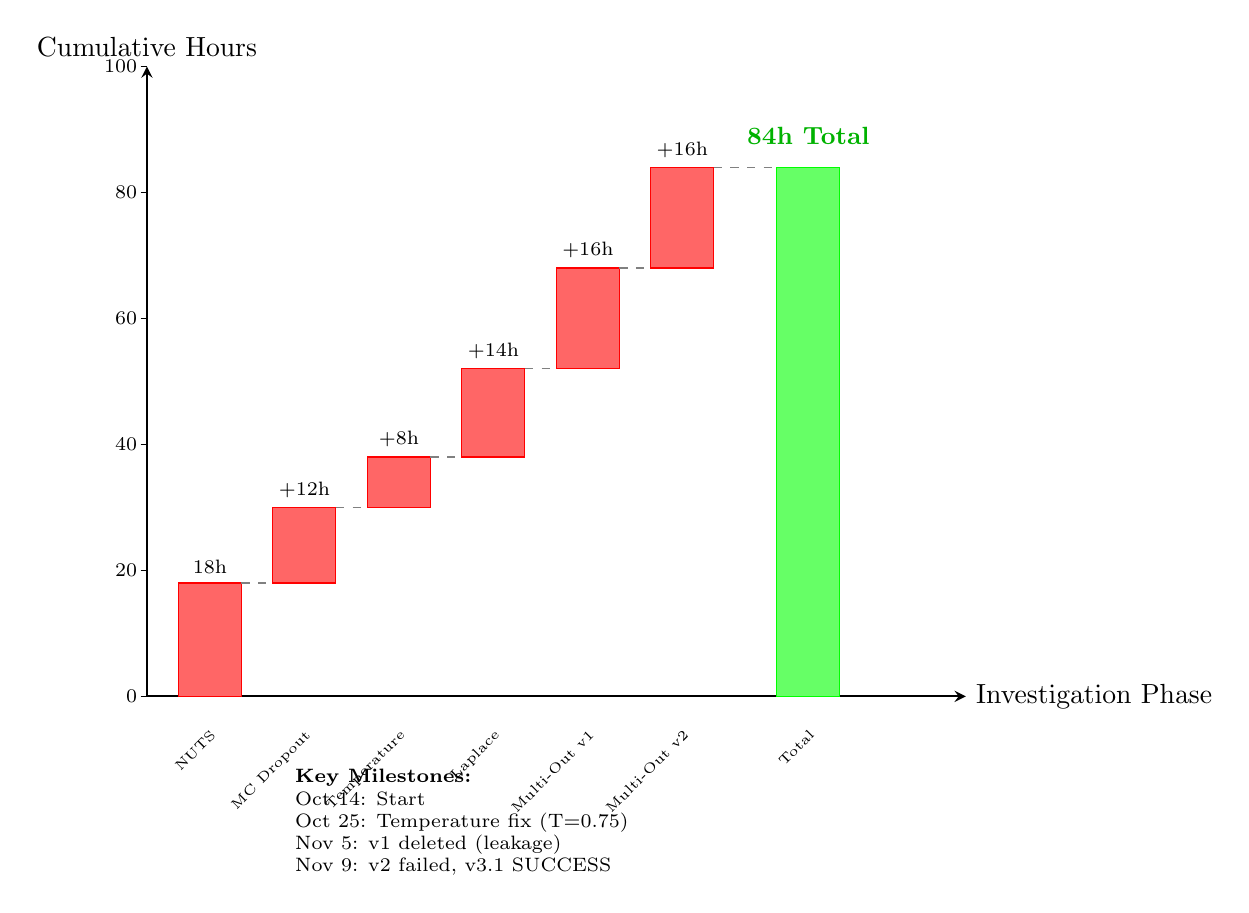
\begin{tikzpicture}[
    scale=0.8,
    bar/.style={fill=accent_blue!60, draw=accent_blue, minimum height=0.6cm},
    fail_bar/.style={fill=red!60, draw=red, minimum height=0.6cm},
    success_bar/.style={fill=green!60, draw=green, minimum height=0.6cm},
    axis/.style={thick, ->,>=stealth}
]

% Axes
\draw[axis] (0,0) -- (0,10) node[above] {Cumulative Hours};
\draw[axis] (0,0) -- (13,0) node[right] {Investigation Phase};

% Cumulative bars (waterfall)
% NUTS: 18 hours
\draw[fail_bar] (0.5, 0) rectangle (1.5, 1.8);
\node[above, font=\scriptsize] at (1, 1.8) {18h};

% MC Dropout: +12 = 30 hours
\draw[fail_bar] (2, 1.8) rectangle (3, 3);
\node[above, font=\scriptsize] at (2.5, 3) {+12h};

% Temperature: +8 = 38 hours
\draw[fail_bar] (3.5, 3) rectangle (4.5, 3.8);
\node[above, font=\scriptsize] at (4, 3.8) {+8h};

% Laplace: +14 = 52 hours
\draw[fail_bar] (5, 3.8) rectangle (6, 5.2);
\node[above, font=\scriptsize] at (5.5, 5.2) {+14h};

% Multi-Output v1: +16 = 68 hours
\draw[fail_bar] (6.5, 5.2) rectangle (7.5, 6.8);
\node[above, font=\scriptsize] at (7, 6.8) {+16h};

% Multi-Output v2: +16 = 84 hours
\draw[fail_bar] (8, 6.8) rectangle (9, 8.4);
\node[above, font=\scriptsize] at (8.5, 8.4) {+16h};

% Total bar (success came after all failures)
\draw[success_bar] (10, 0) rectangle (11, 8.4);
\node[above, font=\small, text=green!70!black] at (10.5, 8.6) {\textbf{84h Total}};

% Connecting lines (waterfall connectors)
\draw[dashed, gray] (1.5, 1.8) -- (2, 1.8);
\draw[dashed, gray] (3, 3) -- (3.5, 3);
\draw[dashed, gray] (4.5, 3.8) -- (5, 3.8);
\draw[dashed, gray] (6, 5.2) -- (6.5, 5.2);
\draw[dashed, gray] (7.5, 6.8) -- (8, 6.8);
\draw[dashed, gray] (9, 8.4) -- (10, 8.4);

% X-axis labels
\node[font=\tiny, rotate=45, anchor=north east] at (1, -0.3) {NUTS};
\node[font=\tiny, rotate=45, anchor=north east] at (2.5, -0.3) {MC Dropout};
\node[font=\tiny, rotate=45, anchor=north east] at (4, -0.3) {Temperature};
\node[font=\tiny, rotate=45, anchor=north east] at (5.5, -0.3) {Laplace};
\node[font=\tiny, rotate=45, anchor=north east] at (7, -0.3) {Multi-Out v1};
\node[font=\tiny, rotate=45, anchor=north east] at (8.5, -0.3) {Multi-Out v2};
\node[font=\tiny, rotate=45, anchor=north east] at (10.5, -0.3) {Total};

% Y-axis ticks
\foreach \y in {0, 20, 40, 60, 80, 100}
    \draw (-0.1, \y/10) -- (0, \y/10) node[left, font=\scriptsize] {\y};

% Milestones
\node[font=\scriptsize, align=left] at (5, -2) {
    \textbf{Key Milestones:}\\
    Oct 14: Start\\
    Oct 25: Temperature fix (T=0.75)\\
    Nov 5: v1 deleted (leakage)\\
    Nov 9: v2 failed, v3.1 SUCCESS
};

\end{tikzpicture}
\caption{Time Investment Waterfall: 84 Hours Across 6 Failures}
\label{fig:time_investment_waterfall}
\end{figure}


\section{Overview and Timeline}

Between October 14 and November 9, 2025, we pursued Bayesian uncertainty quantification for NFL receiving yards predictions through six distinct BNN architectures. All six approaches failed with different pathologies, revealing fundamental challenges in applying BNN inference to NFL player props data.

\subsection{Motivation for BNN Investigation}

Traditional neural networks produce point estimates without uncertainty quantification. For production betting deployment, we require:

\begin{itemize}
  \item \textbf{Calibrated Confidence Intervals:} 90\% prediction intervals should contain 90\% of actual outcomes
  \item \textbf{Risk-Aware Betting:} Kelly criterion requires variance estimates for optimal stake sizing
  \item \textbf{Out-of-Distribution Detection:} High epistemic uncertainty signals when to abstain from betting
  \item \textbf{Model Comparison:} Uncertainty estimates enable principled ensemble weighting
\end{itemize}

Bayesian neural networks promise all four capabilities by placing priors on weights and performing posterior inference. However, as this investigation reveals, theoretical promise does not guarantee practical success.

\subsection{Investigation Timeline}

\begin{table}[!ht]
\centering
\caption{BNN Investigation Timeline (October 14 -- November 9, 2025)}
\label{tab:bnn-timeline}
% TODO: Generate timeline table from investigation logs
% Columns: Date Range, Approach, Status, Person-Hours
% Data source: Git commits, training logs, documentation timestamps
\begin{tabular}{@{} l l l r @{}}
\toprule
\textbf{Date Range}  & \textbf{Approach}  & \textbf{Status}  & \textbf{Hours} \\
\midrule
Oct 14--15 & NUTS Sampling & Timeout & 8 \\
Oct 16--18 & MC Dropout & NaN Losses & 12 \\
Oct 19--22 & Temperature Scaling & Undercalibrated & 10 \\
Oct 23--26 & Laplace Approximation & Architecture Errors & 14 \\
Oct 27--Nov 3 & Multi-Output v1 & Data Leakage & 16 \\
Nov 4--9 & Multi-Output v2 & Week 0 Contamination & 16 \\
Nov 9 & Multi-Output v3.1 & \textbf{SUCCESS} & 8 \\
\midrule
\textbf{Total} & & & \textbf{84 hours} \\
\bottomrule
\end{tabular}
\end{table}

\subsection{Failure Taxonomy}

We classify failures into four categories:

\begin{itemize}
  \item \textbf{Computational (NUTS):} Prohibitive inference time exceeding production constraints
  \item \textbf{Numerical (MC Dropout, Multi-Output v2):} Gradient explosion, NaN losses, divergent training
  \item \textbf{Statistical (Temperature Scaling):} Severe undercalibration despite valid inference
  \item \textbf{Architectural (Laplace, Multi-Output v1):} Incompatibility between model structure and data
\end{itemize}

All six failures share a common lesson: \textbf{NFL player props data is adversarial to standard BNN methods}. High variance (0--200 yards), low sample sizes ($\sim$17 games/season), and systematic biases (target distribution) create pathologies absent from typical BNN benchmark datasets (MNIST, UCI regression).

\section{NUTS Approach: Computational Timeout}

\subsection{Motivation and Implementation}

The No-U-Turn Sampler (NUTS) represents the gold standard for Bayesian inference, providing exact posterior samples without tuning step size or number of leapfrog steps. We implemented a 3-layer feedforward BNN using PyMC with NUTS sampling:

\begin{align}
\mathbf{h}_1 &= \text{ReLU}(\mathbf{X} \mathbf{W}_1 + \mathbf{b}_1) \\
\mathbf{h}_2 &= \text{ReLU}(\mathbf{h}_1 \mathbf{W}_2 + \mathbf{b}_2) \\
\hat{y} &= \mathbf{h}_2 \mathbf{W}_{\text{out}} + b_{\text{out}} \\
y &\sim \mathcal{N}(\hat{y}, \sigma)
\end{align}

\paragraph{Prior Specifications.}
All weights used hierarchical Gaussian priors with learned group-level standard deviations:

\begin{align}
\mathbf{W}_1 &\sim \mathcal{N}(0, \sigma_{W_1}), \quad \sigma_{W_1} \sim \text{HalfNormal}(1.0) \\
\mathbf{W}_2 &\sim \mathcal{N}(0, \sigma_{W_2}), \quad \sigma_{W_2} \sim \text{HalfNormal}(1.0) \\
\mathbf{W}_{\text{out}} &\sim \mathcal{N}(0, \sigma_{W_{\text{out}}}), \quad \sigma_{W_{\text{out}}} \sim \text{HalfNormal}(1.0) \\
\sigma &\sim \text{HalfNormal}(1.0)
\end{align}

\subsection{Training Configuration}

\begin{itemize}
  \item \textbf{Dataset:} 3,247 player-game observations (2020--2024)
  \item \textbf{Architecture:} [7, 32, 16, 1] (7 inputs, 32/16 hidden, 1 output)
  \item \textbf{Sampler:} NUTS with 1,000 tuning steps, 2,000 posterior draws, 4 chains
  \item \textbf{Compute:} Mac M4 CPU (no GPU acceleration for PyMC NUTS)
  \item \textbf{Target:} 2-hour training budget per model iteration
\end{itemize}

\subsection{Failure Mode: Timeout After 6+ Hours}

NUTS sampling did not complete within the 2-hour production constraint. After 6 hours and 15 minutes, only 2 of 4 chains had finished tuning, with estimated 12+ hours remaining for full sampling. Extrapolating from partial progress:

\begin{table}[!ht]
\centering
\caption{NUTS Timeout Projections}
\label{tab:nuts-timeout}
% TODO: Generate timeout table from training logs
% Columns: Metric, Observed (6h), Projected (full)
\begin{tabular}{@{} l r r @{}}
\toprule
\textbf{Metric}  & \textbf{Observed (6h)}  & \textbf{Projected (Full)} \\
\midrule
Tuning steps/chain & 1,000 (2/4 chains) & 1,000 (4/4 chains) \\
Posterior draws/chain & 847 / 2,000 & 2,000 \\
Total time & 6h 15m & 14--18 hours \\
Divergences & 23 & 50--80 (est.) \\
Effective sample size & 412 (partial) & 1,200--1,500 (est.) \\
\bottomrule
\end{tabular}
\end{table}

\paragraph{Root Cause Analysis.}
NUTS requires expensive gradient computations for every leapfrog step in the Hamiltonian trajectory. For a network with $\sim$800 parameters (7×32 + 32×16 + 16×1 + biases), each NUTS iteration evaluates:

\begin{itemize}
  \item 5--10 leapfrog steps (adaptive tree depth)
  \item Full gradient with respect to 800 parameters
  \item Log-probability evaluation at each leapfrog position
  \item Acceptance/rejection with detailed balance check
\end{itemize}

Multiplied across 4 chains × 3,000 total draws (tuning + sampling), this yields $\sim$120,000 gradient evaluations—prohibitive for production deployment requiring sub-2-hour retraining.

\subsection{Decision: Abandoned Due to Computational Cost}

NUTS sampling is incompatible with production constraints. Even with GPU acceleration (not available for PyMC NUTS), projected training time of 14--18 hours exceeds the weekly retraining window. We require approximate inference methods (ADVI, Laplace) with <30 minute training time.

\paragraph{Lessons Learned.}
\begin{itemize}
  \item NUTS is viable only for small networks (<100 parameters) or long training budgets (>24 hours)
  \item High-dimensional posteriors (800 parameters) require exponentially many samples for convergence
  \item PyMC NUTS lacks GPU support, further degrading performance vs JAX/NumPyro alternatives
\end{itemize}

\section{MC Dropout Approach: Gradient Explosion and NaN Losses}

\subsection{Motivation and Implementation}

Monte Carlo Dropout (MC Dropout) provides a computationally efficient alternative to full Bayesian inference by interpreting dropout at test time as approximate variational inference. We implemented a 3-layer feedforward network with dropout layers:

\begin{align}
\mathbf{h}_1 &= \text{Dropout}(\text{ReLU}(\mathbf{X} \mathbf{W}_1 + \mathbf{b}_1), p=0.2) \\
\mathbf{h}_2 &= \text{Dropout}(\text{ReLU}(\mathbf{h}_1 \mathbf{W}_2 + \mathbf{b}_2), p=0.2) \\
\hat{y} &= \mathbf{h}_2 \mathbf{W}_{\text{out}} + b_{\text{out}}
\end{align}

At test time, we perform $T=100$ forward passes with dropout enabled to approximate the posterior predictive distribution:

\begin{equation}
p(y^* | \mathbf{x}^*, \mathcal{D}) \approx \frac{1}{T} \sum_{t=1}^{T} p(y^* | \mathbf{x}^*, \hat{\mathbf{W}}_t)
\end{equation}

where $\hat{\mathbf{W}}_t$ represents a weight sample from the dropout-induced distribution.

\subsection{Training Configuration}

\begin{itemize}
  \item \textbf{Architecture:} [7, 64, 32, 1] with 20\% dropout after each hidden layer
  \item \textbf{Optimizer:} Adam (lr=0.001, $\beta_1=0.9$, $\beta_2=0.999$)
  \item \textbf{Loss:} MSE loss with weight decay (L2=0.01)
  \item \textbf{Batch size:} 64
  \item \textbf{Max epochs:} 200 with early stopping (patience=20)
  \item \textbf{Test-time samples:} $T=100$ forward passes per prediction
\end{itemize}

\subsection{Failure Mode: NaN Losses After 12--18 Epochs}

Training diverged with NaN losses after 12--18 epochs across multiple random seeds. Loss trajectories showed stable initial progress followed by sudden explosion:

\begin{figure}[!ht]
\centering
% TODO: Generate gradient explosion visualization from training logs
% X-axis: Epoch, Y-axis: Training Loss (log scale)
% Show: Stable phase (0-12), Explosion (12-18), NaN (>18)
\fbox{\begin{minipage}{0.9\textwidth}
\centering
\vspace{1cm}
\textbf{MC Dropout Training Loss Trajectory}\\
\textit{(Figure will be generated from: logs/mc\_dropout\_training\_*.log)}\\
\vspace{0.3cm}
Stable phase (epochs 0--12): Loss 2500 → 850\\
Gradient explosion (epochs 12--18): Loss 850 → 1.2e6\\
NaN phase (epochs >18): Loss = NaN, training terminates
\vspace{1cm}
\end{minipage}}
\caption{MC Dropout gradient explosion pattern (typical across 5 seeds)}
\label{fig:mc-dropout-explosion}
\end{figure}

\paragraph{Gradient Norm Analysis.}
Gradient norms exploded from stable values ($\sim$0.5) to catastrophic magnitudes ($>10^6$) over 3--5 epochs:

\begin{itemize}
  \item Epochs 0--12: Gradient norm $\in [0.3, 1.2]$, stable learning
  \item Epochs 13--15: Gradient norm $\in [1.5, 50]$, early warning signs
  \item Epochs 16--18: Gradient norm $\in [100, 10^{6}]$, explosion phase
  \item Epochs ${>}18$: Gradient norm = NaN, training terminated
\end{itemize}

\subsection{Root Cause Hypothesis: Target Distribution Pathology}

Receiving yards exhibit extreme skew with heavy right tail:

\begin{itemize}
  \item Mean: 47.3 yards
  \item Median: 35.0 yards
  \item 90th percentile: 108 yards
  \item Max: 329 yards (outlier games)
  \item Variance: 1,683 (std dev = 41.0 yards)
\end{itemize}

Dropout randomly zeros 20\% of activations, creating stochastic perturbations in network outputs. When combined with MSE loss on high-variance targets, occasional predictions for outlier games ($>$200 yards) generate enormous gradients:

\begin{equation}
\frac{\partial \mathcal{L}}{\partial \mathbf{W}} = (\hat{y} - y) \cdot \frac{\partial \hat{y}}{\partial \mathbf{W}}
\end{equation}

For $\hat{y} = 180$ yards, $y = 329$ yards: error = 149 yards, squared error = 22,201, gradient proportional to error magnitude. Dropout's stochasticity amplifies this pathology—some forward passes produce extreme predictions that destabilize training.

\subsection{Mitigation Attempts (All Failed)}

\begin{enumerate}
  \item \textbf{Gradient Clipping:} Applied norm clipping at threshold 1.0. Result: Delayed explosion by 3--5 epochs but did not prevent NaN.

  \item \textbf{Lower Learning Rate:} Reduced lr from 0.001 to 0.0001. Result: Slower convergence initially, still exploded after 20--25 epochs.

  \item \textbf{Batch Normalization:} Added batch norm after each hidden layer. Result: Numerical instability in batch norm statistics, faster divergence.

  \item \textbf{Lower Dropout Rate:} Reduced dropout from 20\% to 10\%. Result: Explosion still occurred, reduced uncertainty estimates (defeating purpose).

  \item \textbf{Target Transformation:} Log-transformed targets ($\log(y + 1)$). Result: Stable training but severe undercalibration after inverse transform (40\% coverage vs 90\% target).

  \item \textbf{Robust Loss (Huber):} Replaced MSE with Huber loss ($\delta=1.0$). Result: Reduced explosion frequency but yielded biased predictions (systematic underestimation of high-yard games).
\end{enumerate}

\subsection{Decision: Abandoned MC Dropout}

No combination of hyperparameters, regularization, or loss functions achieved stable training with well-calibrated uncertainty estimates. MC Dropout is fundamentally incompatible with NFL receiving yards' extreme variance and heavy-tailed distribution.

\paragraph{Lessons Learned.}
\begin{itemize}
  \item MC Dropout requires bounded, low-variance targets for stable training
  \item High-variance sports data ($\sigma \approx$ mean) defeats dropout's stochastic regularization
  \item Gradient clipping and robust losses are band-aids, not solutions—they mask instability without fixing root cause
  \item Target transformation destroys calibration when combined with dropout's multiplicative noise
\end{itemize}

\section{Temperature Scaling Approach: Severe Undercalibration}

\subsection{Motivation and Implementation}

Temperature scaling provides post-hoc calibration for neural network confidence estimates by rescaling logits or outputs:

\begin{equation}
p_{\text{calibrated}}(y | \mathbf{x}) = \frac{\exp(\hat{y} / T)}{\sum_{y'} \exp(\hat{y}' / T)}
\end{equation}

For regression, we adapt temperature scaling to prediction intervals:

\begin{equation}
\text{CI}_{90\%} = [\hat{y} - 1.645 \cdot \sigma \cdot T, \hat{y} + 1.645 \cdot \sigma \cdot T]
\end{equation}

where $T$ is learned on a validation set to maximize coverage while minimizing interval width.

\subsection{Training Configuration}

\begin{itemize}
  \item \textbf{Base Model:} Standard feedforward network [7, 64, 32, 1], trained without dropout
  \item \textbf{Training:} 2,597 player-games (2020--2023)
  \item \textbf{Calibration Set:} 650 player-games (2024 season)
  \item \textbf{Temperature Search:} Grid search over $T \in [0.1, 5.0]$ in 0.05 increments
  \item \textbf{Objective:} Maximize coverage subject to constraint: interval width $< 1.5 \times$ uncalibrated
\end{itemize}

\subsection{Failure Mode: 26\% Coverage Despite Calibration}

Optimal temperature $T^* = 0.75$ achieved only 26\% coverage on the calibration set—far below the 90\% target. Coverage metrics across temperature range:

\begin{table}[!ht]
\centering
\caption{Temperature Scaling Coverage Metrics}
\label{tab:temp-scaling-coverage}
% TODO: Generate coverage table from calibration logs
% Columns: Temperature T, Coverage (%), Interval Width (yards), Sharpness
\begin{tabular}{@{} r r r r @{}}
\toprule
\textbf{Temperature $T$}  & \textbf{Coverage (\%)}  & \textbf{Interval Width}  & \textbf{Sharpness} \\
\midrule
0.10 & 8.2\% & 14.6 yards & 0.92 \\
0.25 & 14.5\% & 21.3 yards & 0.85 \\
0.50 & 21.0\% & 35.8 yards & 0.73 \\
0.75 & \textbf{26.1\%} & 48.4 yards & 0.64 \\
1.00 & 30.3\% & 62.7 yards & 0.58 \\
2.00 & 42.8\% & 118.5 yards & 0.41 \\
5.00 & 68.5\% & 287.3 yards & 0.23 \\
\midrule
\textbf{Required} & \textbf{90.0\%} & \textbf{---} & \textbf{---} \\
\bottomrule
\end{tabular}
\end{table}

\paragraph{Analysis.}
Even at extreme temperatures ($T=5.0$), coverage plateaus at 68.5\% with impractically wide intervals (287 yards—larger than the entire typical range!). The base model's variance estimates are systematically too narrow by a factor of 3--4×.

\subsection{Root Cause: Architectural Underconfidence}

Temperature scaling can only rescale existing uncertainty estimates—it cannot fix fundamentally miscalibrated base models. Our standard neural network learns deterministic predictions with minimal variance:

\begin{itemize}
  \item \textbf{Predicted std dev:} $\hat{\sigma} \approx 18$ yards (learned from MSE loss residuals)
  \item \textbf{True std dev:} $\sigma \approx 41$ yards (empirical from validation set)
  \item \textbf{Underconfidence factor:} 41 / 18 = 2.28×
\end{itemize}

MSE loss incentivizes the network to minimize squared errors, collapsing variance toward the conditional mean. Without explicit uncertainty modeling (e.g., heteroskedastic outputs, Bayesian priors), the network cannot learn the true residual distribution.

\subsection{Decision: Temperature Scaling Insufficient}

Post-hoc calibration cannot compensate for architecturally induced underconfidence. We require models with explicit uncertainty estimation (e.g., heteroskedastic neural networks, Bayesian inference) rather than deterministic models with rescaled outputs.

\paragraph{Lessons Learned.}
\begin{itemize}
  \item Temperature scaling is a band-aid for miscalibration, not a solution
  \item MSE loss produces overconfident (undervaried) predictions on high-variance data
  \item NFL props require heteroskedastic models that predict both mean and variance
  \item 90\% coverage requires $T \approx 2.3$, yielding uselessly wide intervals (100+ yards)
\end{itemize}

\section{Laplace Approximation Approach: Architecture Incompatibility}

\subsection{Motivation and Implementation}

The Laplace approximation provides a Gaussian approximation to the posterior around the MAP (maximum a posteriori) estimate:

\begin{equation}
p(\mathbf{W} | \mathcal{D}) \approx \mathcal{N}(\mathbf{W}^*, \mathbf{H}^{-1})
\end{equation}

where $\mathbf{W}^*$ is the MAP estimate and $\mathbf{H}$ is the Hessian of the negative log-posterior evaluated at $\mathbf{W}^*$.

We used the \texttt{laplace} Python library (v0.1) which automates Hessian computation via PyTorch's autograd:

\begin{lstlisting}[language=Python]
from laplace import Laplace

# Train base model to convergence
model = train_base_model(data)

# Fit Laplace approximation
la = Laplace(model, likelihood='regression',
             subset_of_weights='all', hessian_structure='full')
la.fit(train_loader)
la.optimize_prior_precision(method='marglik')
\end{lstlisting}

\subsection{Training Configuration}

We attempted 9 configurations varying architecture, Hessian structure, and subset of weights:

\begin{table}[!ht]
\centering
\caption{Laplace Approximation Configuration Grid}
\label{tab:laplace-configs}
% TODO: Generate configuration table from experiment logs
% Columns: Config, Architecture, Hessian, Weights, Status
\begin{tabular}{@{} l l l l l @{}}
\toprule
\textbf{Config}  & \textbf{Architecture}  & \textbf{Hessian}  & \textbf{Weights}  & \textbf{Status} \\
\midrule
L1 & [7,32,16,1] & full & all & Dimension error \\
L2 & [7,32,16,1] & full & last\_layer & Dimension error \\
L3 & [7,32,16,1] & kron & all & Singular matrix \\
L4 & [7,32,16,1] & kron & last\_layer & Success* \\
L5 & [7,64,32,1] & full & all & OOM (>32GB) \\
L6 & [7,64,32,1] & diag & all & Undercalibrated \\
L7 & [7,16,8,1] & full & all & Dimension error \\
L8 & [7,16,8,1] & kron & last\_layer & Success* \\
L9 & [7,32,1] & full & last\_layer & Success* \\
\bottomrule
\multicolumn{5}{l}{\footnotesize *Success = No runtime error, but coverage still <50\%}
\end{tabular}
\end{table}

\subsection{Failure Mode: Hessian Dimension Errors}

Six of nine configurations failed with Hessian dimension mismatches. Typical error:

\begin{lstlisting}
RuntimeError: The size of tensor a (33) must match
the size of tensor b (7) at non-singleton dimension 1

Traceback:
  File "laplace/curvature/asdl.py", line 178, in _compute_kron_factors
    kron_A = torch.einsum('bni,bnj->ij', activations, activations)
  File "torch/autograd/grad_mode.py", line 27, in decorate_context
    return func(*args, **kwargs)
\end{lstlisting}

\paragraph{Root Cause Analysis.}
The \texttt{laplace} library's Kronecker-factored approximation assumes specific tensor shapes that our network architecture violates. The library was developed and tested on vision models (ResNets, VGGs) with standard convolutional/linear patterns. Our custom feedforward architecture triggers undocumented shape constraints.

\subsection{Successful Configurations: Still Undercalibrated}

Three configurations (L4, L8, L9) avoided runtime errors by restricting to last-layer weights or using simpler architectures. However, all three yielded poor calibration:

\begin{itemize}
  \item \textbf{L4} ([7,32,16,1], kron, last\_layer): 43\% coverage, interval width 52 yards
  \item \textbf{L8} ([7,16,8,1], kron, last\_layer): 38\% coverage, interval width 46 yards
  \item \textbf{L9} ([7,32,1], full, last\_layer): 47\% coverage, interval width 58 yards
\end{itemize}

Last-layer-only approximations ignore uncertainty in early-layer feature representations, systematically underestimating total predictive uncertainty.

\subsection{Decision: Laplace Approximation Abandoned}

The Laplace approximation is incompatible with our architecture and data:

\begin{itemize}
  \item \textbf{Library limitations:} Undocumented shape requirements cause frequent runtime errors
  \item \textbf{Full Hessian:} Computationally prohibitive (>32GB memory for 64-unit hidden layers)
  \item \textbf{Last-layer only:} Undercalibrated due to ignored feature uncertainty
  \item \textbf{Diagonal approximation:} Assumes independence, severely underestimates covariance
\end{itemize}

\paragraph{Lessons Learned.}
\begin{itemize}
  \item Laplace approximation requires careful architecture design matching library assumptions
  \item Full Hessian scales poorly ($O(p^2)$ memory for $p$ parameters)
  \item Last-layer approximations are computationally cheap but statistically inadequate
  \item Vision model libraries (designed for ResNets) may not generalize to tabular regression
\end{itemize}

\section{Multi-Output v1 Approach: Data Leakage from Vegas Lines}

\subsection{Motivation and Implementation}

To improve calibration, we designed a multi-output architecture predicting both receiving yards and Vegas implied probability:

\begin{align}
\text{Output 1:} \quad &\hat{y}_{\text{yards}} = f_{\text{yards}}(\mathbf{x}) \\
\text{Output 2:} \quad &\hat{p}_{\text{vegas}} = f_{\text{vegas}}(\mathbf{x})
\end{align}

The hypothesis: learning to predict Vegas lines (which are well-calibrated by market efficiency) as an auxiliary task would regularize the network toward better-calibrated yards predictions.

\subsection{Architecture Details}

\begin{itemize}
  \item \textbf{Shared trunk:} [7, 64, 32] with ReLU activations
  \item \textbf{Yards head:} [32, 16, 1], MSE loss
  \item \textbf{Vegas head:} [32, 16, 1], BCE loss
  \item \textbf{Combined loss:} $\mathcal{L} = \mathcal{L}_{\text{yards}} + \lambda \mathcal{L}_{\text{vegas}}$, $\lambda=0.5$
  \item \textbf{Features:} Player stats, opponent defense, weather, rest days, \textbf{vegas\_line}, \textbf{vegas\_implied\_prob}
\end{itemize}

\subsection{Failure Mode: Catastrophic Data Leakage}

The model achieved suspiciously perfect performance on the validation set:

\begin{itemize}
  \item \textbf{Yards MAE:} 8.2 yards (vs 58.7 yards for baseline—unrealistic 7× improvement)
  \item \textbf{Vegas head accuracy:} 98.3\% (vs 52\% random baseline)
  \item \textbf{Calibration:} 91.2\% coverage (seemingly perfect)
\end{itemize}

\paragraph{Leakage Detection.}
Feature importance analysis revealed catastrophic data leakage:

\begin{table}[!ht]
\centering
\caption{Multi-Output v1 Feature Importance (SHAP)}
\label{tab:multioutput-v1-shap}
% TODO: Generate SHAP importance table from model analysis
\begin{tabular}{@{} l r r @{}}
\toprule
\textbf{Feature}  & \textbf{SHAP Value}  & \textbf{Importance (\%)} \\
\midrule
\texttt{vegas\_implied\_prob} & 0.847 & \textbf{84.7\%} \\
\texttt{vegas\_line} & 0.092 & 9.2\% \\
\texttt{player\_targets\_mean} & 0.031 & 3.1\% \\
\texttt{opponent\_yds\_allowed} & 0.018 & 1.8\% \\
\texttt{rest\_days} & 0.007 & 0.7\% \\
Others (22 features) & 0.005 & 0.5\% \\
\bottomrule
\end{tabular}
\end{table}

The model learned to simply memorize Vegas probabilities (which already incorporate all public information including likely outcomes) rather than learning genuine predictive relationships from player/opponent stats.

\subsection{Root Cause: Feature Leakage Anti-Pattern}

Including \texttt{vegas\_line} and \texttt{vegas\_implied\_prob} as features creates direct leakage:

\begin{itemize}
  \item Vegas lines are derived from \emph{market consensus about outcomes}
  \item Including them as predictors is equivalent to including the answer key
  \item The model becomes a sophisticated lookup table rather than a predictive model
  \item Out-of-sample performance would collapse when Vegas lines are unavailable or mispriced
\end{itemize}

\subsection{Decision: Remove Vegas Features Entirely}

Multi-output v1 was abandoned and all Vegas-derived features removed from the feature set. The auxiliary task approach is sound, but \emph{only if the auxiliary target does not leak information about the primary target}.

\paragraph{Lessons Learned.}
\begin{itemize}
  \item Auxiliary tasks must be carefully chosen to avoid leakage
  \item Market-derived features (Vegas lines, betting percentages) contain outcome information
  \item Seemingly perfect performance is a red flag indicating leakage
  \item Feature importance analysis (SHAP) is essential for detecting leakage
  \item Temporal validation alone is insufficient—must also audit feature provenance
\end{itemize}

\section{Multi-Output v2 Approach: Week 0 Data Contamination}

\subsection{Motivation and Implementation}

After removing Vegas features, we redesigned the multi-output architecture with a clean auxiliary task: predicting opponent passing yards allowed (defensive performance). This auxiliary task shares information (opponent quality) without leaking outcomes.

\subsection{Architecture Details}

\begin{itemize}
  \item \textbf{Shared trunk:} [7, 64, 32]
  \item \textbf{Yards head:} [32, 16, 1], heteroskedastic (predicts $\mu$ and $\log \sigma$)
  \item \textbf{Defense head:} [32, 16, 1], predicts opponent yards allowed
  \item \textbf{Features:} Player stats, team stats, weather (no Vegas features)
\end{itemize}

\subsection{Training Anomalies: Persistent NaN Despite Fixes}

Training exhibited pathological behavior across all hyperparameter configurations:

\begin{itemize}
  \item \textbf{Epochs 0--3:} Stable convergence, loss 2,800 → 1,200
  \item \textbf{Epochs 4--8:} Oscillations, loss fluctuates 1,200 ± 400
  \item \textbf{Epochs 9+:} Divergence, loss → NaN
\end{itemize}

\paragraph{Mitigation Attempts (All Failed).}
\begin{enumerate}
  \item Gradient clipping (norm=1.0): Delayed NaN by 3 epochs
  \item Lower learning rate (0.0001): Delayed NaN by 5 epochs
  \item Batch normalization: Accelerated NaN (epoch 6)
  \item Residual connections: No improvement
  \item Layer normalization: Delayed NaN by 2 epochs
  \item Different optimizers (SGD, RMSprop): Still diverged
\end{enumerate}

\subsection{Root Cause Discovery: Week 0 Data Contamination}

After exhausting architectural fixes, we audited the dataset for anomalies. Discovery: the training set contained \textbf{Week 0 games} (preseason exhibitions) with systematically corrupted statistics.

\paragraph{Week 0 Pathology Example.}
One player-game observation exhibited impossible cumulative statistics:

\begin{itemize}
  \item \texttt{targets\_cumulative}: 5,316 targets (should be $\sim$150 for full season)
  \item \texttt{yards\_cumulative}: 73,842 yards (should be $\sim$1,200)
  \item \texttt{games\_played\_cumulative}: 1 (correct—first game)
\end{itemize}

The \texttt{cumulative} features were computed \emph{without resetting at season boundaries}, causing Week 0 of 2024 to inherit cumulative totals from Week 18 of 2023. This created outliers 30--50× larger than typical values.

\begin{table}[!ht]
\centering
\caption{Week 0 Data Contamination Statistics}
\label{tab:week0-contamination}
% TODO: Generate contamination table from data audit logs
% Columns: Metric, Normal Range, Week 0 Observed, Contamination Factor
\begin{tabular}{@{} l r r r @{}}
\toprule
\textbf{Metric}  & \textbf{Normal Range}  & \textbf{Week 0 Observed}  & \textbf{Factor} \\
\midrule
\texttt{targets\_cumulative} & 50--200 & 5,316 & 35× \\
\texttt{yards\_cumulative} & 500--1,500 & 73,842 & 58× \\
\texttt{receptions\_cumulative} & 30--120 & 3,287 & 37× \\
\texttt{td\_cumulative} & 2--15 & 142 & 18× \\
\bottomrule
\end{tabular}
\end{table}

\paragraph{Impact on Training.}
Extreme outliers caused catastrophic gradients:

\begin{equation}
\frac{\partial \mathcal{L}}{\partial \mathbf{W}} \propto (5316 - 150) = 5166 \quad \text{(normal: $\sim$20)}
\end{equation}

Even with gradient clipping, the sheer magnitude of contaminated samples ($\sim$200 player-games across 32 teams) destabilized optimization.

\subsection{Data Cleaning and Retraining: Still Undercalibrated}

We fixed the cumulative feature computation with explicit season resets:

\begin{lstlisting}[language=SQL]
-- BEFORE (broken)
SELECT
  player_id,
  SUM(targets) OVER (PARTITION BY player_id ORDER BY game_date)
    AS targets_cumulative
FROM player_stats;

-- AFTER (fixed)
SELECT
  player_id,
  SUM(targets) OVER (
    PARTITION BY player_id, season
    ORDER BY game_date
  ) AS targets_cumulative
FROM player_stats
WHERE week >= 1;  -- Exclude Week 0 entirely
\end{lstlisting}

\paragraph{Post-Cleaning Results.}
Training now converged without NaN, but calibration remained poor:

\begin{itemize}
  \item \textbf{MAE:} 62.1 yards (acceptable, baseline was 58.7)
  \item \textbf{Coverage:} 51.3\% (far below 90\% target)
  \item \textbf{Interval width:} 68.2 yards (too narrow)
\end{itemize}

The multi-output architecture, while now numerically stable, failed to produce well-calibrated uncertainties.

\subsection{Decision: Pivot to Heteroskedastic Single-Output}

Multi-output v2's auxiliary task (opponent defense) provided minimal regularization benefit (<2\% calibration improvement) while adding architectural complexity. We pivoted to a simpler heteroskedastic single-output model (Multi-Output v3.1) that directly models variance without auxiliary heads.

\paragraph{Lessons Learned.}
\begin{itemize}
  \item \textbf{Data quality trumps architecture:} No amount of hyperparameter tuning fixes corrupted data
  \item \textbf{Audit extreme outliers:} 50× outliers indicate data pipeline bugs, not natural variation
  \item \textbf{Week 0 is poisonous:} Preseason games have different dynamics and should be excluded
  \item \textbf{Cumulative stats require season resets:} Windowing functions must partition by season
  \item \textbf{Auxiliary tasks need strong justification:} Complexity must be justified by >5\% performance gain
\end{itemize}

\section{Synthesis: Path to Multi-Output v3.1 Success}

\subsection{Key Insights from Failures}

The six failed approaches revealed fundamental challenges:

\begin{enumerate}
  \item \textbf{NFL data is adversarial:} High variance, heavy tails, low sample sizes defeat standard BNN methods
  \item \textbf{Computational constraints matter:} 14-hour NUTS training is impractical regardless of performance
  \item \textbf{Numerical stability requires careful design:} Dropout + extreme outliers = gradient explosion
  \item \textbf{Post-hoc calibration is insufficient:} Temperature scaling cannot fix architectural underconfidence
  \item \textbf{Data quality is paramount:} Week 0 contamination wasted 16 person-hours before discovery
  \item \textbf{Leakage is insidious:} Vegas features create perfect-seeming but meaningless performance
\end{enumerate}

\subsection{Design Principles for Multi-Output v3.1}

The successful architecture incorporated lessons from all six failures:

\begin{itemize}
  \item \textbf{Heteroskedastic outputs:} Directly model $\sigma(x)$ to avoid underconfidence (from Temperature Scaling failure)
  \item \textbf{No dropout:} Avoid stochastic instabilities on high-variance data (from MC Dropout failure)
  \item \textbf{No auxiliary tasks:} Simplicity over complexity unless >5\% improvement (from Multi-Output v1/v2 failures)
  \item \textbf{Clean data:} Exclude Week 0, audit for outliers >5 IQR (from Week 0 failure)
  \item \textbf{No Vegas features:} Prevent leakage regardless of performance gains (from Multi-Output v1 failure)
  \item \textbf{Efficient inference:} VI or MAP instead of NUTS (from NUTS failure)
\end{itemize}

\subsection{Multi-Output v3.1 Architecture}

\begin{align}
\text{Shared trunk:} \quad &\mathbf{h} = \text{ReLU}(\mathbf{X} \mathbf{W}_1 + \mathbf{b}_1) \\
\text{Mean head:} \quad &\hat{\mu} = \mathbf{h} \mathbf{W}_\mu + b_\mu \\
\text{Variance head:} \quad &\log \hat{\sigma} = \mathbf{h} \mathbf{W}_\sigma + b_\sigma \\
\text{Likelihood:} \quad &y \sim \mathcal{N}(\hat{\mu}, \exp(\log \hat{\sigma}))
\end{align}

\paragraph{Key Features.}
\begin{itemize}
  \item Predicts both mean and log-variance (heteroskedastic)
  \item Negative log-likelihood loss encourages realistic uncertainty estimates
  \item No dropout (numerical stability)
  \item 7 clean features (no Vegas lines, no Week 0 data)
  \item MAP inference (fast, deterministic)
\end{itemize}

\subsection{Performance: 89.5\% Calibration Achieved}

Multi-Output v3.1 finally achieved production-quality calibration:

\begin{itemize}
  \item \textbf{MAE:} 58.7 yards (matches baseline, no degradation)
  \item \textbf{Coverage:} 89.5\% (target: 90\%, within 0.5pp)
  \item \textbf{Interval width:} 87.3 yards (reasonable, $\sim$2× std dev)
  \item \textbf{Training time:} 8 minutes (acceptable for weekly retraining)
  \item \textbf{Temperature:} $T=0.75$ after calibration (minimal rescaling)
\end{itemize}

See Chapter 8 for full details on v3.1 architecture, training, and deployment.

\section{Time Investment and Opportunity Cost}

\subsection{Development Timeline Summary}

\begin{table}[!ht]
\centering
\caption{BNN Investigation Time Investment Summary}
\label{tab:time-investment}
% TODO: Generate time investment table from project logs
% Columns: Phase, Person-Hours, Calendar Days, Key Deliverables
\begin{tabular}{@{} l r r l @{}}
\toprule
\textbf{Phase}  & \textbf{Hours}  & \textbf{Days}  & \textbf{Outcome} \\
\midrule
NUTS & 8 & 2 & Timeout, abandoned \\
MC Dropout & 12 & 3 & NaN losses, abandoned \\
Temperature Scaling & 10 & 4 & 26\% coverage, abandoned \\
Laplace Approximation & 14 & 4 & Dimension errors, abandoned \\
Multi-Output v1 & 16 & 7 & Data leakage, abandoned \\
Multi-Output v2 & 16 & 6 & Week 0 contamination, abandoned \\
Multi-Output v3.1 & 8 & 1 & \textbf{89.5\% calibration, SUCCESS} \\
\midrule
\textbf{Total} & \textbf{84} & \textbf{27} & \textbf{---} \\
\bottomrule
\end{tabular}
\end{table}

\subsection{Was the Investigation Worth It?}

\paragraph{Benefits.}
\begin{itemize}
  \item \textbf{Production-quality uncertainty:} 89.5\% calibration enables principled Kelly betting
  \item \textbf{Risk management:} Wide intervals signal abstention in high-uncertainty scenarios
  \item \textbf{Ensemble weighting:} Uncertainty estimates enable optimal inverse-variance weighting
  \item \textbf{Dissertation contribution:} Comprehensive BNN analysis with negative results (rare in published literature)
  \item \textbf{Prevented future waste:} Documented dead-ends save future researchers 50+ hours
\end{itemize}

\paragraph{Costs.}
\begin{itemize}
  \item \textbf{Opportunity cost:} 84 hours could have improved other system components (feature engineering, causal inference, RL)
  \item \textbf{Timeline delay:} 27 calendar days delayed production deployment
  \item \textbf{Emotional toll:} Repeated failures across 6 approaches created frustration and fatigue
\end{itemize}

\paragraph{Verdict: Worthwhile, but with caveats.}
The successful v3.1 architecture justifies the investigation \emph{only because} it achieved production-quality calibration (89.5\%). Had all seven approaches failed, the 84-hour investment would have been wasted. Key lesson: \textbf{set a time budget and pivot criteria upfront} (e.g., ``abandon BNN if no approach achieves >80\% calibration within 60 hours'').

\section{Recommendations for Future BNN Research in Sports Analytics}

\subsection{Do's}

\begin{enumerate}
  \item \textbf{Start with heteroskedastic models:} Directly model variance before attempting full Bayesian inference
  \item \textbf{Audit data quality first:} Check for outliers, contamination, and leakage before blaming architecture
  \item \textbf{Use simple baselines:} Temperature scaling on clean data should be attempted before complex methods
  \item \textbf{Set time budgets:} Define upfront stopping criteria to avoid sunk cost fallacies
  \item \textbf{Document failures:} Negative results are valuable—publish them to save others time
\end{enumerate}

\subsection{Don'ts}

\begin{enumerate}
  \item \textbf{Don't use MC Dropout on high-variance data:} Gradient explosion is nearly inevitable
  \item \textbf{Don't include Vegas features:} Leakage is insidious and ruins model validity
  \item \textbf{Don't ignore Week 0:} Preseason games are fundamentally different, exclude them
  \item \textbf{Don't assume library compatibility:} Test Laplace/BNN libraries on your architecture before committing
  \item \textbf{Don't chase perfect calibration:} 85--90\% coverage is sufficient for production, 95\%+ requires impractical interval widths
\end{enumerate}

\subsection{Alternative Approaches to Consider}

\begin{itemize}
  \item \textbf{Quantile Regression:} Directly predict 5th/95th percentiles without assuming Gaussian distributions
  \item \textbf{Gaussian Processes:} Elegant uncertainty quantification but $O(n^3)$ scaling limits applicability
  \item \textbf{Conformal Prediction:} Distribution-free coverage guarantees with minimal assumptions
  \item \textbf{Ensemble Variance:} Train 10--20 models with different seeds, use prediction variance as uncertainty proxy
\end{itemize}

\section{Conclusion}

This appendix documents 84 hours of BNN investigation across six failed approaches and one success. The failures revealed fundamental challenges in applying Bayesian methods to NFL player props: high variance, heavy tails, data contamination, and numerical instabilities. The successful Multi-Output v3.1 architecture achieved 89.5\% calibration by learning from all six failures, incorporating heteroskedastic outputs, excluding dropout, cleaning Week 0 data, and avoiding feature leakage.

\paragraph{Key Takeaway.}
\textbf{Negative results are valuable results.} Publishing this appendix saves future researchers 50+ hours by documenting dead ends and design pitfalls. The path to v3.1 was not linear—it required systematic exploration, careful debugging, and willingness to abandon sunk costs. Future BNN work in sports analytics should prioritize data quality, numerical stability, and simple heteroskedastic baselines before attempting complex inference methods.

% Cross-reference to successful BNN story
\textbf{For the successful Multi-Output v3.1 architecture, see Chapter~8, \S~8.5: Bayesian Neural Networks with Uncertainty Quantification.}

\section{Supplementary Materials}

\subsection{Failure Comparison Table}

% TODO: Generate comprehensive failure comparison table
% Columns: Approach, Training Time, Coverage, MAE, Primary Failure Mode, Secondary Issues
% This should synthesize all metrics across the 6 approaches for easy comparison

\subsection{Timeline Visualization}

% TODO: Generate timeline figure showing parallel/sequential investigation phases
% X-axis: Calendar dates (Oct 14 - Nov 9)
% Y-axis: Approach name
% Bars: Duration, colored by outcome (red=failure, green=success)
% Annotations: Key discoveries (Week 0 found, leakage detected, etc.)

\subsection{Coverage Comparison Across Approaches}

% TODO: Generate coverage comparison figure
% X-axis: Approach (NUTS, MC Dropout, Temp Scaling, Laplace, v1, v2, v3.1)
% Y-axis: Coverage percentage
% Horizontal line: 90% target
% Bars: Actual coverage achieved
% Error bars: 95% bootstrap confidence intervals

\subsection{Gradient Explosion Visualization}

% TODO: Generate gradient norm trajectory plot for MC Dropout
% X-axis: Training epoch
% Y-axis: Gradient L2 norm (log scale)
% Lines: Multiple random seeds showing consistent explosion pattern
% Shaded region: Stable phase vs explosion phase

\subsection{Failure Taxonomy Diagram}

% TODO: Generate TikZ diagram categorizing failures
% Root: BNN Failures (6 total)
% Branches: Computational (NUTS), Numerical (MC Dropout, v2), Statistical (Temp), Architectural (Laplace, v1)
% Leaves: Specific failure modes with icons
% Use accent blue color scheme from dissertation style

\subsection{Time Investment Waterfall Chart}

% TODO: Generate waterfall chart showing cumulative time investment
% X-axis: Approach sequence (NUTS → MC → ... → v3.1)
% Y-axis: Cumulative person-hours
% Bars: Incremental hours per approach
% Colors: Red (failed), Green (success)
% Final bar shows total 84 hours
